\documentclass[]{article}
\hyphenation{co-rres-pon-dien-tes te-ner E-ben-sper-ger de-pre-da-do-res dis-po-ni-ble be-ne-fi-cio-sa in-di-vi-dual so-cia-li-dad mos-tra-ron fuen-tes a-cep-ta-ble ta-ma-ño o-pues-ta mo-de-lo es-tu-dian-tes e-jer-ci-cios co-rres-pon-dien-te mo-di-fi-ca-dos mo-di-fi-car-lo ma-ni-pu-lar}
\usepackage{amssymb,amsmath}
\usepackage{ifxetex,ifluatex}
\ifxetex
  \usepackage{fontspec,xltxtra,xunicode}
  \defaultfontfeatures{Mapping=tex-text,Scale=MatchLowercase}
\else
  \ifluatex
    \usepackage{fontspec}
    \defaultfontfeatures{Mapping=tex-text,Scale=MatchLowercase}
  \else
    \usepackage[utf8]{inputenc}
  \fi
\fi
\usepackage{color}
\usepackage{fancyvrb}
\DefineShortVerb[commandchars=\\\{\}]{\|}
\DefineVerbatimEnvironment{Highlighting}{Verbatim}{commandchars=\\\{\}}
% Add ',fontsize=\small' for more characters per line
\newenvironment{Shaded}{}{}
\newcommand{\KeywordTok}[1]{\textcolor[rgb]{0.00,0.44,0.13}{\textbf{{#1}}}}
\newcommand{\DataTypeTok}[1]{\textcolor[rgb]{0.56,0.13,0.00}{{#1}}}
\newcommand{\DecValTok}[1]{\textcolor[rgb]{0.25,0.63,0.44}{{#1}}}
\newcommand{\BaseNTok}[1]{\textcolor[rgb]{0.25,0.63,0.44}{{#1}}}
\newcommand{\FloatTok}[1]{\textcolor[rgb]{0.25,0.63,0.44}{{#1}}}
\newcommand{\CharTok}[1]{\textcolor[rgb]{0.25,0.44,0.63}{{#1}}}
\newcommand{\StringTok}[1]{\textcolor[rgb]{0.25,0.44,0.63}{{#1}}}
\newcommand{\CommentTok}[1]{\textcolor[rgb]{0.38,0.63,0.69}{\textit{{#1}}}}
\newcommand{\OtherTok}[1]{\textcolor[rgb]{0.00,0.44,0.13}{{#1}}}
\newcommand{\AlertTok}[1]{\textcolor[rgb]{1.00,0.00,0.00}{\textbf{{#1}}}}
\newcommand{\FunctionTok}[1]{\textcolor[rgb]{0.02,0.16,0.49}{{#1}}}
\newcommand{\RegionMarkerTok}[1]{{#1}}
\newcommand{\ErrorTok}[1]{\textcolor[rgb]{1.00,0.00,0.00}{\textbf{{#1}}}}
\newcommand{\NormalTok}[1]{{#1}}
\usepackage{graphicx}
% We will generate all images so they have a width \maxwidth. This means
% that they will get their normal width if they fit onto the page, but
% are scaled down if they would overflow the margins.
\makeatletter
\def\maxwidth{\ifdim\Gin@nat@width>\linewidth\linewidth
\else\Gin@nat@width\fi}
\makeatother
\let\Oldincludegraphics\includegraphics
\renewcommand{\includegraphics}[1]{\Oldincludegraphics[width=\maxwidth]{#1}}
\ifxetex
  \usepackage[setpagesize=false, % page size defined by xetex
              unicode=false, % unicode breaks when used with xetex
              xetex,
              colorlinks=true,
              linkcolor=blue]{hyperref}
\else
  \usepackage[unicode=true,
              colorlinks=true,
              linkcolor=blue]{hyperref}
\fi
\hypersetup{breaklinks=true, pdfborder={0 0 0}}
\setlength{\parindent}{0pt}
\setlength{\parskip}{6pt plus 2pt minus 1pt}
\setlength{\emergencystretch}{3em}  % prevent overfull lines
\setcounter{secnumdepth}{0}


\begin{document}

\section{Ejercicio de programación VI: Estructuras de Control}

\subsubsection{{[}IMSER 2013{]}}

De otros años:

\begin{itemize}
\item
  Cambiar parte d del útimo parcial: si el bus tiene el máximo de
  pasajeros no sube a más nadie y si tiene el mínimo (0) no baja nadie.
\item
  Crecimiento exponencial \ldots{}?
\item
  Caminata del borracho?
\item
  Símil función preg?
\item
  Loops con errores: un while que es infinito, un for que tiene mal
  puesto el rango, \ldots{}
\end{itemize}
\begin{center}\rule{3in}{0.4pt}\end{center}

\subsection{1. Conteos por fila}

\subsubsection{1.a Loop for}

Suponga que usted debe analizar regularmente matrices de datos,
obtenidos en muestreos sucesivos, con cantidades de filas variables. Una
de las tareas que se le pide realizar cotidianamente es hacer un conteo
de la cantidad de valores mayores a 45 \emph{por cada fila} de la
matriz. Para no tener que hacerlo manualmente, usted decide que lo mejor
es crear un script de R con el cual hacer este conteo automáticamente.

Para hacer el script lo mejor es usar una matriz de juguete con la cual
hacer pruebas. Para esto sirven las siguientes líneas (que también se
encuentran en el script del ejercicio):

\begin{Shaded}
\begin{Highlighting}[]
\CommentTok{# Generación de la matriz datos:}
\NormalTok{datos <- }\KeywordTok{matrix}\NormalTok{(}\KeywordTok{rpois}\NormalTok{(}\KeywordTok{rpois}\NormalTok{(}\DecValTok{1}\NormalTok{, }\DecValTok{125}\NormalTok{) * }\DecValTok{15}\NormalTok{, }\DecValTok{43}\NormalTok{), }\DataTypeTok{ncol =} \DecValTok{15}\NormalTok{)}
\end{Highlighting}
\end{Shaded}
Para lograr su objetivo, usted deberá usar un loop \texttt{for}, con el
cual completará el vector \texttt{out}, el cual contendrá las sumas de
valores mayores a 45 por filas. Como un mini ejemplo, si su matriz
\texttt{datos} es la siguiente:

\begin{Shaded}
\begin{Highlighting}[]
\NormalTok{datos <- datos[}\DecValTok{1}\NormalTok{:}\DecValTok{5}\NormalTok{, }\DecValTok{1}\NormalTok{:}\DecValTok{5}\NormalTok{]}
\NormalTok{datos}
\end{Highlighting}
\end{Shaded}
\begin{verbatim}
##      [,1] [,2] [,3] [,4] [,5]
## [1,]   33   35   47   48   41
## [2,]   49   34   43   56   52
## [3,]   38   53   54   30   44
## [4,]   50   51   31   31   38
## [5,]   34   47   44   44   44
\end{verbatim}
Entonces el vector \texttt{out} será así:

\begin{Shaded}
\begin{Highlighting}[]
\NormalTok{out}
\end{Highlighting}
\end{Shaded}
\begin{verbatim}
## [1] 2 3 2 2 1
\end{verbatim}
(Este es un ejemplo creado con números al azar, por supuesto.)

Nótese que el sistema de corrección espera que haya un \texttt{for} en
el script (naturalmente) y que la \emph{variable de iteración} (ver
lección 6.2) tome como valores \textbf{números enteros positivos}.

\subsubsection{1.b Extra: apply}

Luego de hacer el script del ejercicio 1.a, usted se da cuenta que lo
mismo se puede hacer y de forma ``más elegante'' con una función
\texttt{apply}. Para esto usted deduce que debe crear una función propia
capaz de contar la cantidad de valores mayores a 45 (o a un valor
variable, si usted lo prefiere) de un vector numérico cualquiera y luego
aplicar esta función con \texttt{apply} a todas las filas de
\texttt{datos} (note que cada fila es un vector cuando se las trata por
separado).

Para completar el ejercicio deberá simplemente usar \texttt{apply} para
lograr el mismo vector \texttt{out} que en el ejercicio 1.a.

\begin{center}\rule{3in}{0.4pt}\end{center}

\subsection{2. todavía no se bien que}

\subsubsection{2.a Zenón recargado}

Hacer un while para encontrar el n para un valor arbitrario de
$\varepsilon$, siguiendo las directivas del ejercicio de zenon.R

Como seguramente recordará, en el Repartido I se propuso calcular la
serie que representa a la
\href{https://es.wikipedia.org/wiki/Paradojas\_de\_Zen\%C3\%B3n\#La\_dicotom.C3.ADa}{paradoja
de Zenón}, cuyo valor para el enésimo elemento se definió como:

\[
  Z_n = \sum_{i=1}^{i=n} \frac{1}{2 ^ i} \;=\;
  \frac{1}{2 ^ 1} + \frac{1}{2 ^ 2} + \frac{1}{2 ^ 3} + ... + \frac{1}{2 ^ n} \;=\;
  \frac{1}{2} + \frac{1}{4} + \frac{1}{8} + ... + \frac{1}{2 ^ n}
\]

En R, el valor de $Z_n$ se puede obtener con las siguientes líneas de
código:

\begin{Shaded}
\begin{Highlighting}[]
\NormalTok{n <- }\DecValTok{20}  \CommentTok{# El n puede ser cualquiera en verdad...}
\NormalTok{Zn <- }\KeywordTok{sum}\NormalTok{(}\DecValTok{1}\NormalTok{/(}\DecValTok{2}\NormalTok{^(}\DecValTok{1}\NormalTok{:n)))}
\end{Highlighting}
\end{Shaded}
En ocasión de aquel primer repartido, el objetivo era encontrar el
mínimo \texttt{n} que cumpliera la desigualdad $1 - Z_n < \varepsilon$,
siendo $\varepsilon = 10 ^ {-6}$. El único método con que contaba en ese
momento era manualmente cambiar el valor de \texttt{n} aumentando en una
unidad, ejecutar el código y determinar manualmente si cumplía tal
condición (para repetir el proceso en caso de que de no hacerlo). Sin
embargo con las herramientas que usted a aprendido en esta unidad es
posible ver que se pueden automatizar estos procedimientos, e incluso
generalizarlo para cualquier $\varepsilon$. Este es el objetivo de este
ejercicio.

Para esto usted deberá usar el loop \texttt{while}, ya que es (en
principio) el más adecuado para esta tarea, pues no sabemos de antemano
cual va a ser el \texttt{n} ``correcto''. Además recuerde que el loop
\texttt{while} necesita que se cumpla una condición para continuar su
ejecución, tal como el procedimiento de encontrar el \texttt{n}
correcto.

La siguiente es la salida en la consola para el caso de
\texttt{epsilon \textless{}- 5e-2}:

\begin{verbatim}
## n = 2 - Zn = 0.75 
## n = 3 - Zn = 0.875 
## n = 4 - Zn = 0.9375 
## n = 5 - Zn = 0.9688
\end{verbatim}
\textbf{Recuerde que}: \textbf{1.} en cada iteración \texttt{n} debe
aumentar en una unidad, \textbf{2.} el script debe funcionar igual
debien para cualquier valor de \texttt{epsilon} elegido y \textbf{3.}
debe utilizar el código indicado anteriormente para obtener \texttt{Zn}
o la corrección automática tendrá problemas con el redondeo de los
valores.

\subsubsection{2.b Guardar los valores}

Puede usar for o while, da lo mismo

\begin{verbatim}
## n = 2 - Zn = 0.75 
## n = 3 - Zn = 0.875 
## n = 4 - Zn = 0.9375 
## n = 5 - Zn = 0.9688
\end{verbatim}
\begin{verbatim}
## [1] 5
\end{verbatim}
\begin{verbatim}
## [1] 0.03125
\end{verbatim}
\begin{figure}[htbp]
\centering
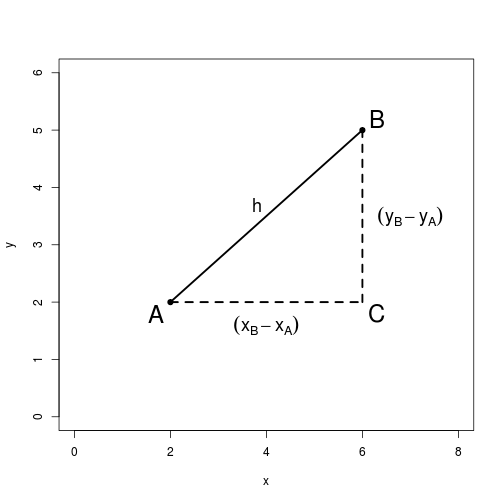
\includegraphics{figure/unnamed-chunk-7.png}
\caption{Serie de Zenón, con n = 5}
\end{figure}

Nota: en el ejemplo de

\begin{center}\rule{3in}{0.4pt}\end{center}

\section{Parcial II}

\paragraph{Curso IMSER 2012}

\subsection{Instrucciones:}

En el archivo
``\href{http://eva.universidad.edu.uy/file.php/1454/ejercicios\_de\_programacion/parcial-II.R}{parcial-II.R}''
ud. tiene un script en el cual deberá guardar todos los comandos del
ejercicio, siguiendo la demarcación que se muestra en el mismo.

Nota: los ejercicios del parcial son dependientes de los anteriores en
el sentido de que utilizan objetos creados, pero no implica que no se
puedan tratar de resolver independientemente.

Los ejercicios con (\texttt{*}) presentan un puntaje de 1.5, mientras
que los que no tienen (\texttt{*}) equivalen a 1 punto.

Una vez terminado el parcial usted deberá subir a la
\href{http://eva.universidad.edu.uy/mod/assignment/view.php?id=102998}{página
del EVA} el archivo ``parcial-II.R'' con su código.

\begin{center}\rule{3in}{0.4pt}\end{center}

\subsection{Letra}

Para simular la cantidad de pasajeros de un ómnibus urbano se ha creado
el código que aparece sobre el final del ejercicio (y que también se
encuentra en el script parcial-II.R). El criterio es el siguiente: el
bus recorre 25 paradas, empezando el trayecto sin pasajeros. En cada
parada se subirá una cantidad aleatoria de entre 0 a 6 personas (siendo
todas las cantidades equiprobables), pero debido a que existe un máximo
estipulado de 44 pasajeros, a partir del momento en que se alcanza ese
valor el vehículo deja de subir gente.

\begin{center}\rule{3in}{0.4pt}\end{center}

\subsubsection{(\texttt{*}) a. Código incompleto}

Completar el código: las líneas en blanco que se encuentran dentro de
los límites del código indican en dónde debe cambiarse. \textbf{El resto
de las líneas están correctas}.

Código fuente:

\begin{Shaded}
\begin{Highlighting}[]
\CommentTok{# Preparación:}
\NormalTok{paradas <- }\DecValTok{25}
\NormalTok{pasajeros <- }\DecValTok{0}
\NormalTok{## <<}
\NormalTok{registro[}\DecValTok{1}\NormalTok{] <- pasajeros}
\NormalTok{for (i in }\DecValTok{1}\NormalTok{:paradas) \{}
    \NormalTok{## << A ver si no se llenó:}
    \NormalTok{if (pasajeros >= }\DecValTok{44}\NormalTok{) }
        \NormalTok{\{}
            \CommentTok{# Ajuste por si llega a 44 antes de terminar:}
            \NormalTok{registro[i:paradas] <- }\DecValTok{44}
            \KeywordTok{cat}\NormalTok{(}\StringTok{"Bus lleno!}\CharTok{\textbackslash{}n}\StringTok{"}\NormalTok{)  }\CommentTok{# Mensaje de aviso...}
            \NormalTok{break}
        \NormalTok{\}  }\CommentTok{# <- este no estaba}
    \NormalTok{## << Si no se corta el loop, se agrega un nuevo registro:}
    \NormalTok{registro[i] <- pasajeros}
    \CommentTok{# Para ir viendo cuánto hay:}
    \KeywordTok{cat}\NormalTok{(}\StringTok{"Parada"}\NormalTok{, i, }\StringTok{"hay"}\NormalTok{, pasajeros, }\StringTok{"pasajeros}\CharTok{\textbackslash{}n}\StringTok{"}\NormalTok{)}
\NormalTok{\}}
\KeywordTok{plot}\NormalTok{(registro, }\DataTypeTok{xlab =} \StringTok{"Parada"}\NormalTok{, }\DataTypeTok{ylab =} \StringTok{"No. de pasajeros"}\NormalTok{)}
\end{Highlighting}
\end{Shaded}
Sugerencias: (1) la función \texttt{sample} puede ser útil para simular
la subida de pasajeros. (2) Tanto en este como en los siguientes
ejercicios, en caso de no estar seguro/a de cómo proceder, puede
facilitar mucho la tarea hacer un diagrama de flujo sencillo antes de
empezar a escribir código.

La siguiente imagen se obtuvo haciendo la simulación, ejecutando
previamente \texttt{set.seed(11)} y luego el comando gráfico:

\begin{Shaded}
\begin{Highlighting}[]
\KeywordTok{plot}\NormalTok{(registro, }\DataTypeTok{xlab =} \StringTok{"Parada"}\NormalTok{, }\DataTypeTok{ylab =} \StringTok{"No. de pasajeros"}\NormalTok{)}
\end{Highlighting}
\end{Shaded}
\begin{figure}[htbp]
\centering
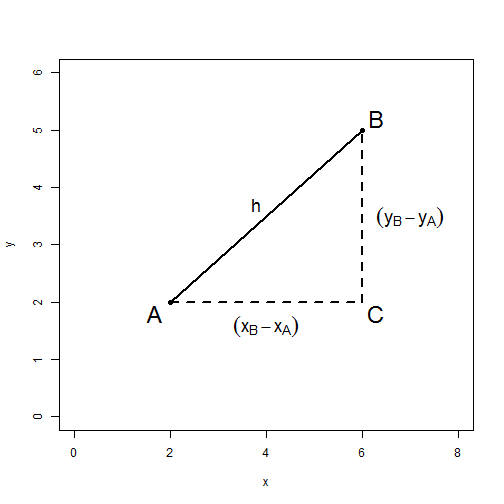
\includegraphics{figure/unnamed-chunk-10.png}
\caption{plot of chunk unnamed-chunk-10}
\end{figure}

\begin{center}\rule{3in}{0.4pt}\end{center}

\subsubsection{b. Cambio de loop}

Modifique el código de la parte anterior de forma tal que haga lo mismo,
pero utilizando un loop \texttt{while}.

Sugerencias: (1) agrege manualmente una variable (p.ej.: \texttt{i}) que
sirva para indexar los distintos objetos y recuerde actualizarla en la
linea correcta del código y (2) usar un \texttt{if} posterior al loop
puede ser útil para sustituir los ceros del final por 44 en el vector
registro (aunque no es de ninguna manera el único método).

Nota: el gráfico que se dió en la parte anterior tamibén aplica para
este ejercicio.

\subsubsection{(\texttt{*}) c. Función \texttt{bus}}

Modifique el código reparado en la parte \textbf{a} para crear una
función llamada \texttt{bus} que ejecute la misma simulación, en la que
el número de paradas y capacidad máxima del bus sean los argumentos de
la misma. El nombre de estos argumentos son a su elección.

Como salida la función debe devolver simplemente el vector
\texttt{registro}.

Nota: recuerde que esta función debe trabajar correctamente para
cualquier elección del número de paradas y máximo de pasajeros. En el
siguiente ejemplo se muestra un caso que puede servir de referencia:

\begin{Shaded}
\begin{Highlighting}[]
\KeywordTok{set.seed}\NormalTok{(}\DecValTok{11}\NormalTok{)}
\CommentTok{# Nro. de paradas = 40 Máximo de pasajeros = 80}
\NormalTok{x <- }\KeywordTok{bus}\NormalTok{(}\DecValTok{40}\NormalTok{, }\DecValTok{80}\NormalTok{)}
\end{Highlighting}
\end{Shaded}
\begin{verbatim}
## Parada 1 hay 1 pasajeros
## Parada 2 hay 1 pasajeros
## Parada 3 hay 4 pasajeros
## Parada 4 hay 4 pasajeros
## Parada 5 hay 4 pasajeros
## Parada 6 hay 10 pasajeros
## Parada 7 hay 10 pasajeros
## Parada 8 hay 12 pasajeros
## Parada 9 hay 18 pasajeros
## Parada 10 hay 18 pasajeros
## Parada 11 hay 19 pasajeros
## Parada 12 hay 22 pasajeros
## Parada 13 hay 28 pasajeros
## Parada 14 hay 33 pasajeros
## Parada 15 hay 38 pasajeros
## Parada 16 hay 42 pasajeros
## Parada 17 hay 45 pasajeros
## Parada 18 hay 47 pasajeros
## Parada 19 hay 48 pasajeros
## Parada 20 hay 51 pasajeros
## Parada 21 hay 52 pasajeros
## Parada 22 hay 56 pasajeros
## Parada 23 hay 58 pasajeros
## Parada 24 hay 60 pasajeros
## Parada 25 hay 60 pasajeros
## Parada 26 hay 63 pasajeros
## Parada 27 hay 65 pasajeros
## Parada 28 hay 65 pasajeros
## Parada 29 hay 65 pasajeros
## Parada 30 hay 67 pasajeros
## Parada 31 hay 70 pasajeros
## Parada 32 hay 72 pasajeros
## Parada 33 hay 74 pasajeros
## Parada 34 hay 75 pasajeros
## Bus lleno!
\end{verbatim}
\begin{figure}[htbp]
\centering
\includegraphics{figure/unnamed-chunk-12.png}
\caption{plot of chunk unnamed-chunk-12}
\end{figure}

\begin{center}\rule{3in}{0.4pt}\end{center}

\subsubsection{d. Gente que también baja}

Hacer una variante del código (de cualquiera de las partes anteriores)
en la que además de subir personas, a partir de la parada 10 se bajen
entre 1 y 5 pasajeros por parada. Tanto la subida y la bajada deben
ejecutarse \textbf{antes} de determinar si se alcanzó el máximo
estipulado de pasajeros y por lo tanto si debe dejar de detenerse el bus
en las paradas.

Sugerencia: puede ser muy útil hacer un diagrama de flujo sencillo para
planificar el código antes de escribirlo.

El siguiente es un ejemplo del resultado de aplicar los cambios que se
piden en la función \texttt{bus}:

\begin{Shaded}
\begin{Highlighting}[]
\KeywordTok{set.seed}\NormalTok{(}\DecValTok{11}\NormalTok{)}
\NormalTok{x <- }\KeywordTok{bus}\NormalTok{(}\DecValTok{30}\NormalTok{, }\DecValTok{60}\NormalTok{)}
\end{Highlighting}
\end{Shaded}
\begin{verbatim}
## Parada 1 hay 1 pasajeros
## Parada 2 hay 1 pasajeros
## Parada 3 hay 4 pasajeros
## Parada 4 hay 4 pasajeros
## Parada 5 hay 4 pasajeros
## Parada 6 hay 10 pasajeros
## Parada 7 hay 10 pasajeros
## Parada 8 hay 12 pasajeros
## Parada 9 hay 18 pasajeros
## Parada 10 hay 17 pasajeros
## Parada 11 hay 15 pasajeros
## Parada 12 hay 16 pasajeros
## Parada 13 hay 17 pasajeros
## Parada 14 hay 18 pasajeros
## Parada 15 hay 19 pasajeros
## Parada 16 hay 21 pasajeros
## Parada 17 hay 22 pasajeros
## Parada 18 hay 23 pasajeros
## Parada 19 hay 22 pasajeros
## Parada 20 hay 21 pasajeros
## Parada 21 hay 20 pasajeros
## Parada 22 hay 16 pasajeros
## Parada 23 hay 18 pasajeros
## Parada 24 hay 16 pasajeros
## Parada 25 hay 14 pasajeros
## Parada 26 hay 12 pasajeros
## Parada 27 hay 14 pasajeros
## Parada 28 hay 16 pasajeros
## Parada 29 hay 13 pasajeros
## Parada 30 hay 15 pasajeros
\end{verbatim}
\begin{figure}[htbp]
\centering
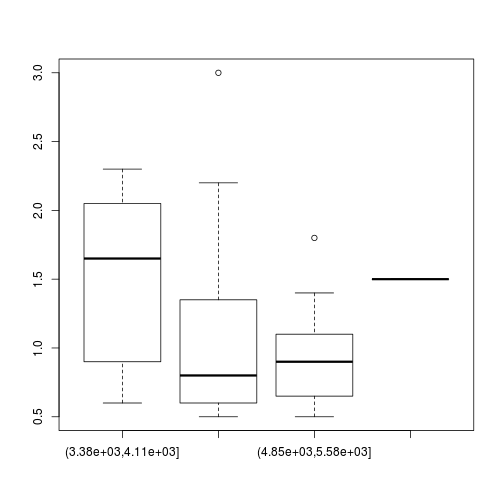
\includegraphics{figure/unnamed-chunk-14.png}
\caption{plot of chunk unnamed-chunk-14}
\end{figure}

\end{document}
